\hypertarget{para_8cpp}{\section{Dokumentacja pliku para.\-cpp}
\label{para_8cpp}\index{para.\-cpp@{para.\-cpp}}
}


Funkcje klasy para.  


{\ttfamily \#include \char`\"{}para.\-h\char`\"{}}\\*
Wykres zależności załączania dla para.\-cpp\-:\nopagebreak
\begin{figure}[H]
\begin{center}
\leavevmode
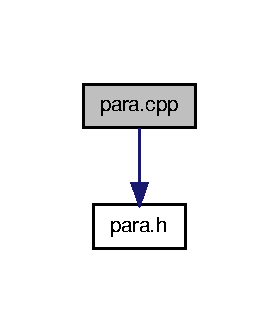
\includegraphics[width=134pt]{para_8cpp__incl}
\end{center}
\end{figure}
